\chapter{Konzeption}
\label{Konzeption}

Dieses Kapitel beschreibt die Resultate und Ergebnisse aus der Konzeptionsphase. Nachfolgend werden auf die verschiedenen Konzeptionsvarianten eingegangen. Dabei werden Überlegungen und Bezüge zur Aufgabenstellung gemacht. Jede Variante wird abschliessend mit eienm kurzen Fazit beurteilt.

\section{Konzeptionsgrundlage}
Als Konzeptionsgrundlage dient das Pflichtenheft, welches im Anhang \todo{referenz} einsehbar ist. Wie darin erwähnt, soll das Modul möglichst frei drehend konzipiert werden. Dies ist das ausschlaggebendste Kriterium für die Bauform des Moduls. Da der Velodyne VLP-16, wie in Kapitel \todo{ref} erläutert, einen begrenzten horizontalen Öffnungswinkel besitzt, wurde bei den folgenden Konzepten die Möglichkeit eines beweglichen Moduls geprüft. Ein weiteres relevantes Kriterium ist die Einsatzmöglichkeit des Modul. Es soll einerseits auf dem Packbot, sowie auch als eigenständiges Produkt funktionieren. Daher sind als Schnittstellen einen Speiseanschluss, welcher 12 Volt DC liefert und eine Ethernet RJ45-Anschluss nötig. Nachfolgend sind auf diesen Grundlagen drei Varianten dargelegt.


\section {Variante 1: Plattform}
\label{var1}
Die Variante 1: Plattform ist in der Skizze in Abbildung \todo{referenz} ersichtlich. Bei dieser Konstruktion werden alle elektronischen Komponenten, welche für die Signalverarbeitung und die Energieversorgung nötig sind, in einem rechteckigen Gehäuse im unteren Teil verbaut. Die Interface Box des Velodyne VLP-16 wird auch in diesem Gehäuse untergebracht. Lediglich der Laserscanner VLP-16 befindet sich ausserhalb des Gehäuses auf der Plattform oberhalb des Gehäuses.
	
 Die Eigenheit dieser Konzeption ist die Plattform, auf welcher sich der Velodyne VLP-16 befindet. Der Einsatz dieser Plattform erklärt sich durch ein bekanntes Regelungsexperiment namens "Ball on a Plate". In Abbildung \todo{ref }ist eine CAD-Zeichnung eines solchen Regelungsexperiment dargestellt. Bei "Ball on a Plate" werden zwei Servomotoren, welche je mit einem Gelenk mit einer Seite der Plattform verbunden sind, angesteuert. Indem die Servomotoren mittig auf der Seite mit der rechteckigen Plattform verbunden sind, kann durch Drehen der Servomotoren die Plattform zweiachsig geneigt werden. Im Regelungsexperiment kann durch Zuhilfenahme einer PID-Regelung ein Ball darauf balanciert werden. 
 
\begin{figure}[H]
	\centering
 	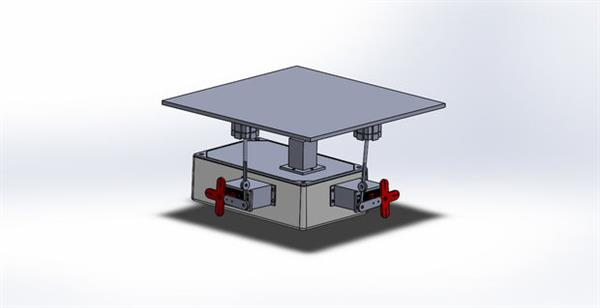
\includegraphics[width=1\textwidth]{resources/ballonaplate_cad}
	\caption{Ball on a Plate CAD {\cite{3ders.org}}}
	\label{fig:BalllonaPlateCAD}
\end{figure} 

 Diese Überlegungen bieten die Möglichkeit den Laserscanner VLP-16, welcher in der Konzeption auf der Plattform befestigt ist, durch das ansteuern der Servomotoren in alle Richtungen zu neigen. Somit kann  der Öffnungswinkel in jede Richtung vergrößert werden. Die Grenzen liegen dabei in der Begrenzung.
 
 Hauptproblematik bei dieser Konzeption ist die zusätzlich nötige Sensorik. Durch die Neigung der Plattform kann ohne zusätzliche Sensorik nicht auf die Transformationsebenen zurückgeschlossen werden. Dies erschwert die Visualisierung der 3D-Laserscanner Messdaten. Die Plattform müsste mittels einer eigenen IMU, welche aus Gyrosensor, Accelerometer und Magnetometer besteht, erweitert werden.
 
 Während der Besprechung mit Herr Jensen vom blabla \todo{ZEIT} wurde diese Konzeption verworfen und nicht mehr weiter betrachtet.
 
 
 
 \textbf{Fazit}
 

\section {Variante 2: Turm}
\label{var2}



\section {ausgewählte Komponenten}

\section{Zwischenfazit}
\label{Zwischenfazit_konzept}
